\documentclass[../Bachelorarbeit.tex]{subfiles}
\begin{document}

\subsection{Kontextanalyse}
Ziel der Kontextanalyse ist die Abgrenzung des Kontexts \bzw das Finden von Systemgrenzen. Bei dem mehrachsigen Positioniersystem handelt es sich um ein sogenanntes eingebettetes System (\eng Embedded System). Diese kommunizieren meist stark mit ihrer Umwelt \bzw sind meist stark mit dieser verankert. % Quelle
So auch hat das Positioniersystem Schnittstellen, über die eine Kommunikation mit Nachbarsystemen stattfindet. In der Systemkonzeption muss folglich geklärt werden, wo genau die Systemgrenzen liegen. Weiterhin findet in der Kontextabgrenzung auch die Identifizierung von Nachbarsystemen statt.\\ % Quelle
Zuerst muss geklärt werden, ob die Systemumgebung dynamischer natur ist, das heißt, dass Nachbarsysteme wechseln \bzw das System nicht umgebungstreu ist. Handelt es sich im Gegensatz dazu um ein System mit stabiler Umgebung, ist die Darstellung von Nachbarsystemen simpel und kann nachfolgend im entsprechenden Diagramm dokumentiert werden. Da das mehrachsige Positioniersystem fest in den Laborraum integriert ist, und alle Nachbarsysteme bereits bekannt sind, wird in der Analyse von einer statischen Umgebung ausgegangen. Die sich anschließende Liste zeigt alle derzeitigen Nachbarsysteme, in die das mehrachsige Positioniersystem eingebettet ist.\\

\begin{itemize}
    \item Laborcomputer
    \item Ablageschale/Aufnahmeschale (Ablagepositionen)
    \item Externe Industriesteuerungen
    \item Augmented Reality Server
    \item Verwaltungsschalen (Digitaler Zwilling)
    \item mögliche spätere Erweiterung: Förderbänder
    \item mögliche spätere Erweiterung: Vorratslager (statt Aufnahmeschale)
    \item mögliche spätere Erweiterung: Lagermagazin(e) (statt Ablageschale)
\end{itemize}

Ist die Identifizierung der Nachbarsysteme abgeschlossen, kann mit der Kontextanalyse begonnen werden. Der Kontext unterteilt sich in den logischen Kontext und den physikalischen Kontext. Der \textbf{logische Kontext} betrachtet die Kommunikation mit den Nachbarsystemen, wohingegen der \textbf{physikalische Kontext} auf die Kommunikationshardware fokussiert ist.\\ % Quelle
Für die Dokumentation der logischen Kontextabgrenzung bietet sich sich das Anwendungsfalldiagramm der UML (Unified Modeling Language) an. Dabei handelt es sich um die allgemein gängige Form für diese Aufgabe. Das Anwendungsfalldiagramm ist geeignet an dieser Stelle für die Modellierung, da für die Darstellung noch keine detaillierten Entscheidungen über die Schnittstellen getroffen werden müssen. Es besitzt die Fähigkeit das zu modellierende System und seine Nachbarsysteme in Beziehung darzustellen und deren Kommunikation grundlegend anzudeuten. \autoref{fig:my-img1} zeigt die logische Kontextabgrenzung des mehrachsigen Positioniersystems zu den bereits aufgezählten Nachbarsystemen mittels des Anwendungsfalldiagramms.

\begin{figure}[h]
    \centering
    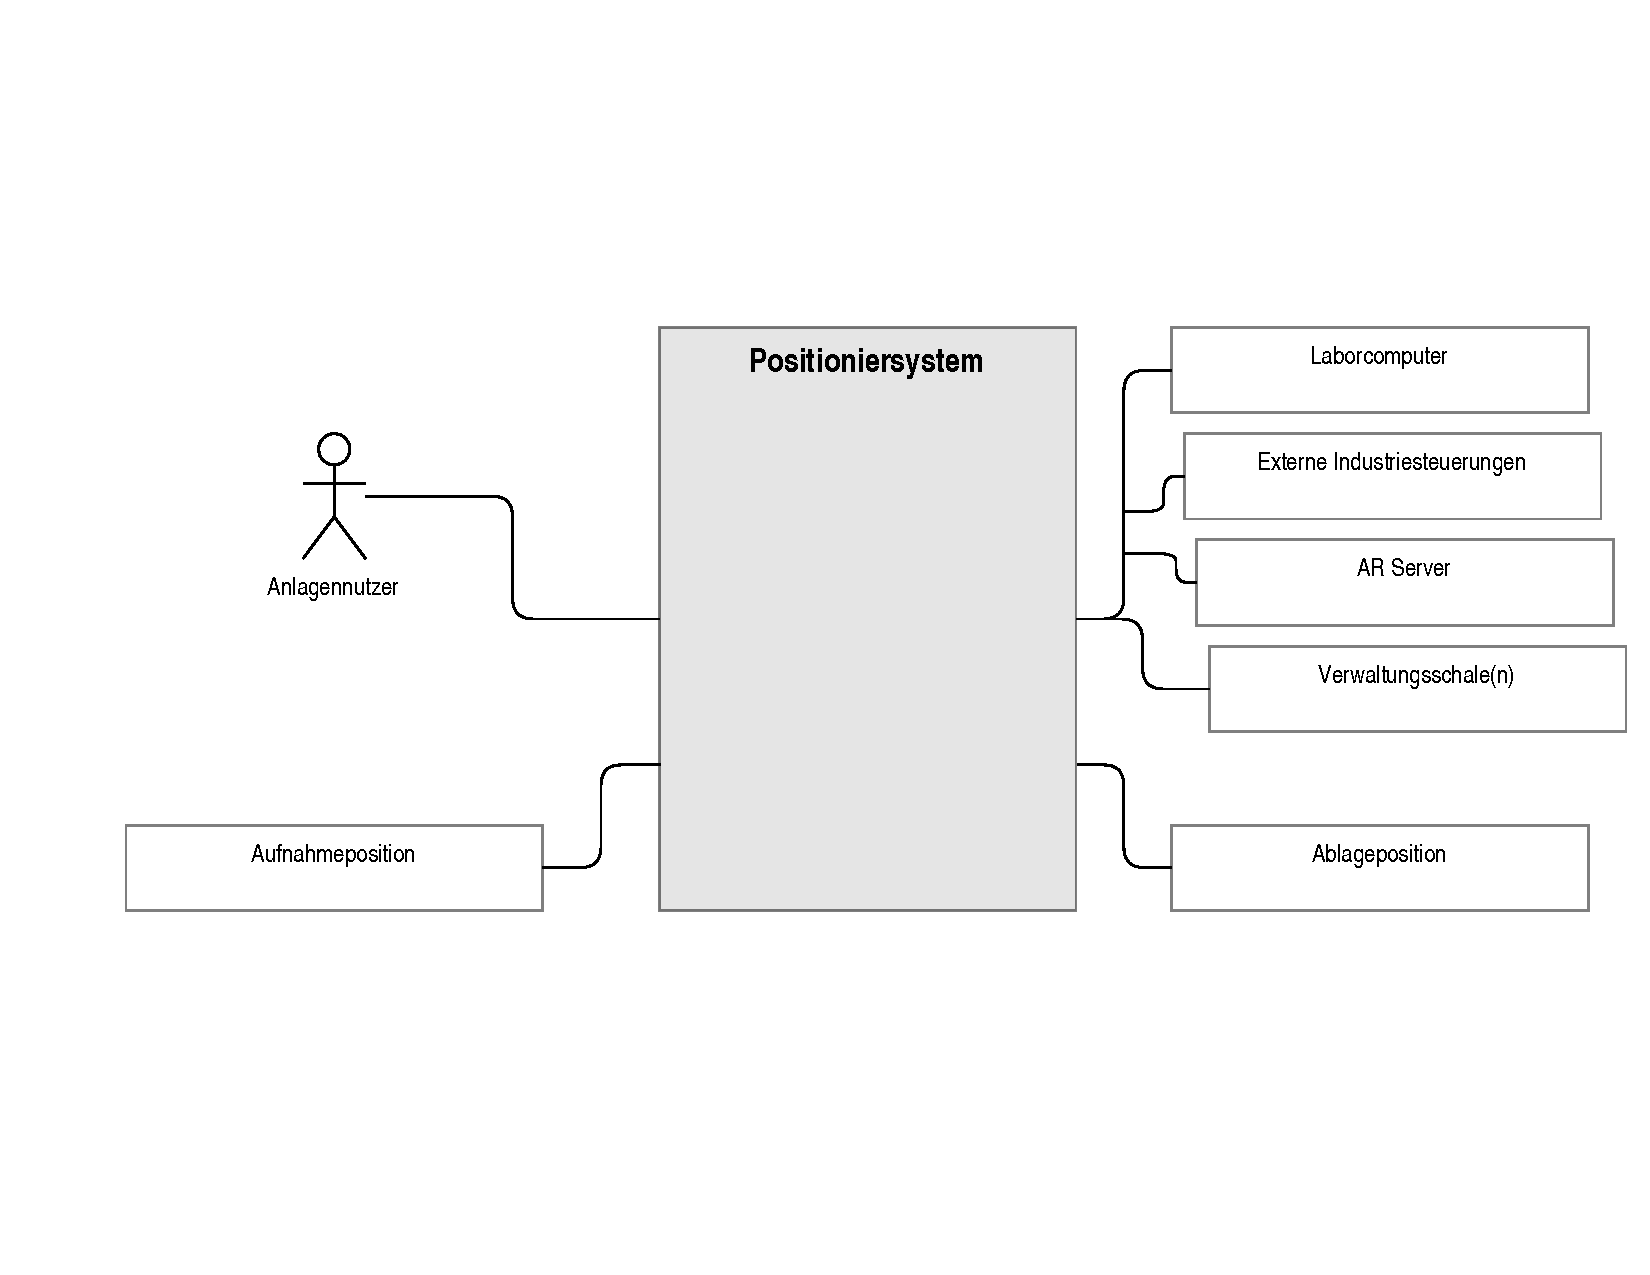
\includegraphics[width=\textwidth]{Images/kontextana.pdf}
    \caption[Logische Kontextabgrenzung]{Logische Kontextabgrenzung des mehrachsigen Positioniersystems}
    \label{fig:my-img1}
\end{figure}

Noch nicht erwähnt waren bisher die Akteure des Positioniersystems. Akteure eines eingebetteten Systems sind Sensoren, E/A-Geräte, Nachbarsysteme und die Zeit. Sie befinden sich grundsätzlich außerhalb des Systems. \\ % Quelle
Die zu modellierende Laboranlage besitzt folglich mehrere Nachbarsysteme, die als Akteure bezeichnet werden können. Weiterhin sind Menschen, die in Kontakt mit dem System stehen, relevant. Diese gelten auch als Akteure und werden als Strichfigur im Anwendungsfalldiagramm aufgenommen. Der Anlagennutzer des Positioniersystems ist als Akteur auf der linken Seite der \autoref{fig:my-img1} aufgeführt. Die Nachbarsysteme auf der rechten oberen Seite besitzen wiederum Akteure, die an dieser Stelle jedoch nicht dargestellt sind, da diese mit dem mehrachsigen Positioniersystem nur indirekt über die Nachbarsysteme kommunizieren.\\
Es kann abschließend festgehalten werden, dass der logische Kontext beantwortet, welche Akteure für das System existieren. Es besteht die Notwendigkeit nach diesen zu suchen, und sie in Form des Anwendungsfalldiagrammes im Bezug zum Positioniersystem darzustellen.\\
Nach der Aufstellung des logischen Kontexts der Laboranlage wird nun darauf aufbauend fortgesetzt mit der physikalischen Kontextabgrenzung. Im unterschied zum logischen Kontext wird die Fragestellung erweitert um die konkreten Einflüsse der Akteure auf das System. Es gilt zu untersuchen, wie die Kommunikation zwischen den Akteuren und dem mehrachsigen Positioniersystem aufgebaut ist. Dazu bietet es sich an das Verteilungsdiagramm der UML zu nutzen. Wie auch schon bei der logischen Kontextabgrenzung wird das System Positioniereinheit im Zentrum zwischen den Akteuren als zentraler Knoten dargestellt. Die Nachbarsysteme werden ringsherum als eigenständige Knoten aufgeführt. In der fogenden Abbildung der physikalischen Kontextabgrenzung wird auch der Anlagennutzer als Nachbarsystem betrachtet, um mehr Freiräume in der Darstellung der Schnittstelle zwischen diesem und dem Positioniersystem zu ermöglichen. \autoref{fig:my-img2} zeigt das Verteildiagramm der Positioniereinehit und seiner Nachbarsysteme zur Beantwortung der Frage nach dem physikalischen Kontext.\\

\begin{figure}[h]
    \centering
    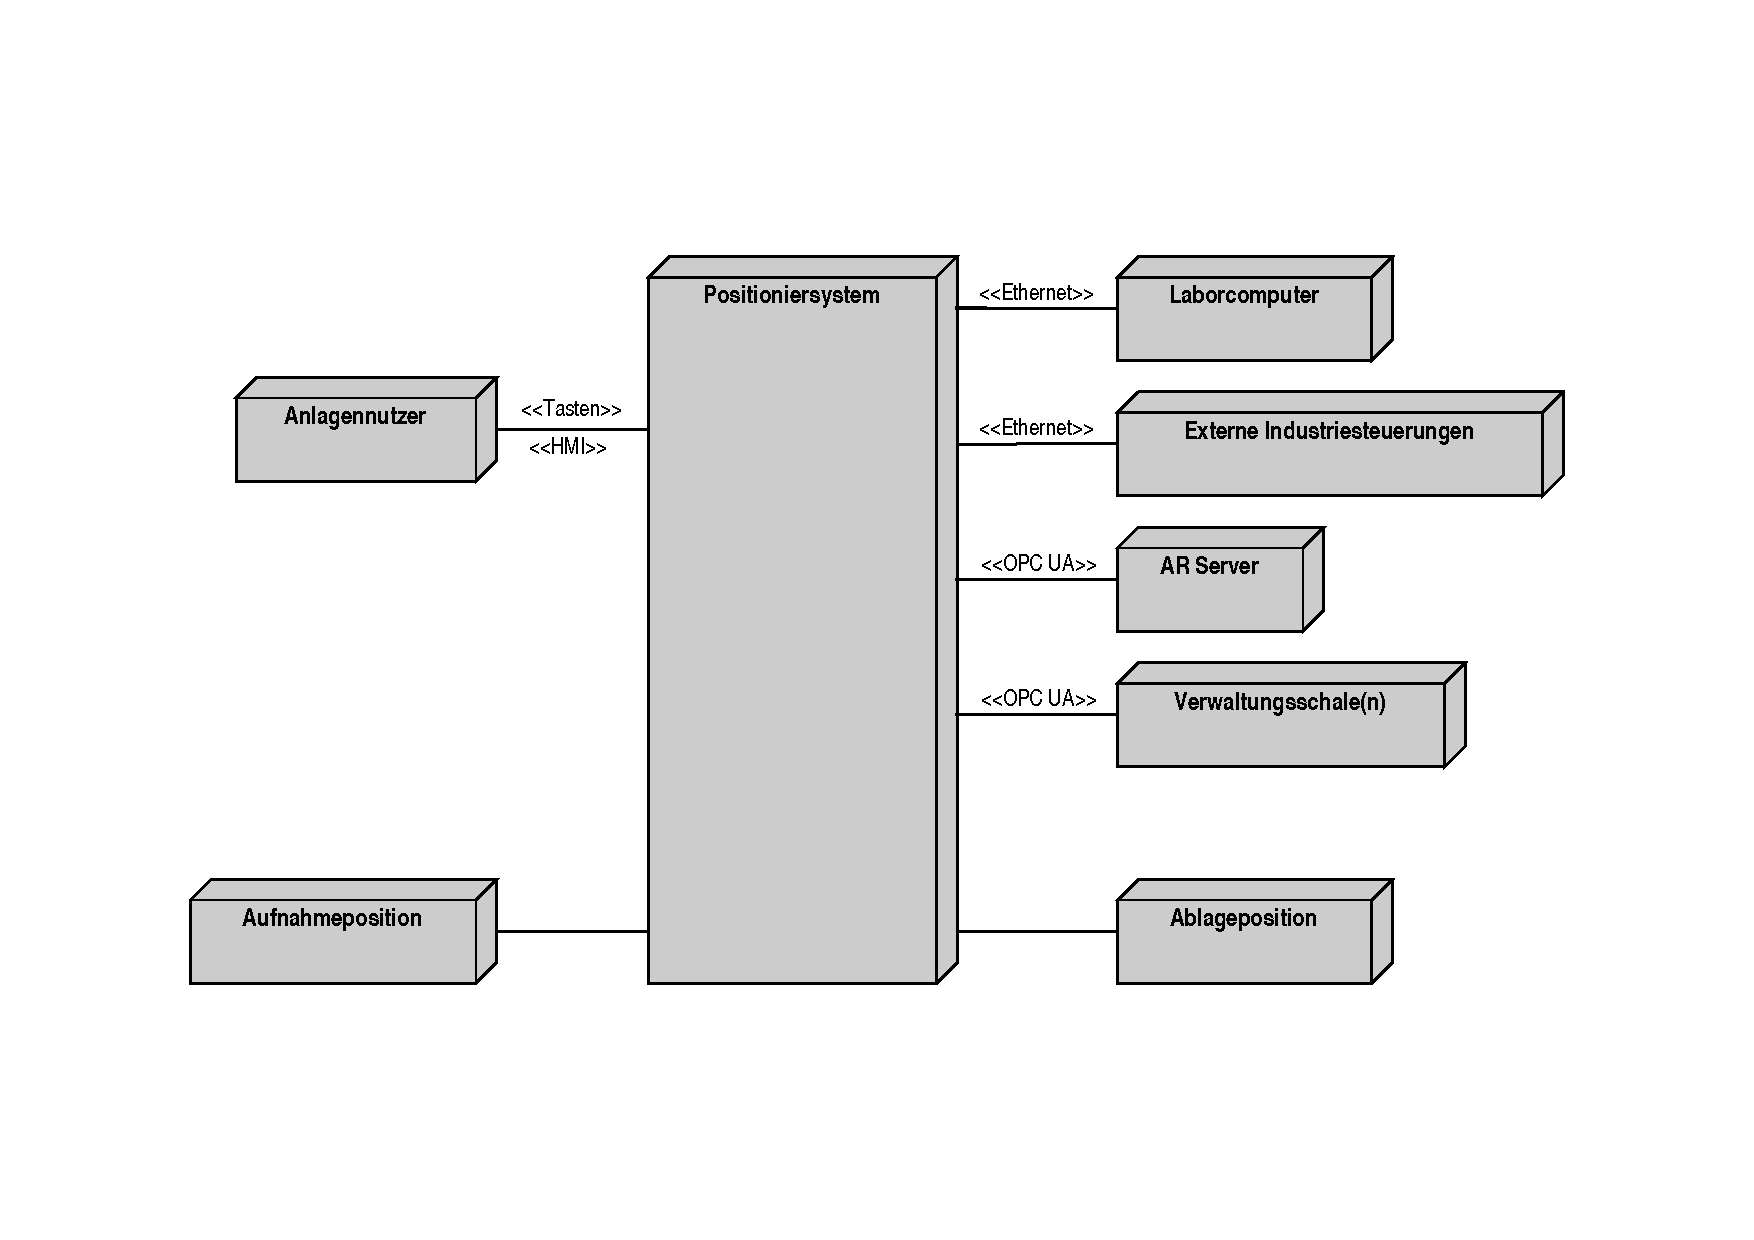
\includegraphics[width=\textwidth]{Images/phys_abgrenzung.pdf}
    \caption[Physikalische Kontextabgrenzung]{Physikalische Kontextabgrenzung des mehrachsigen Positioniersystems}
    \label{fig:my-img2}
\end{figure}

Im unterschied zu \autoref{fig:my-img2} werden nun an den Verbindungen zwischen den Systemen Stereotypen mit aufgeführt, falls die Hardware und Kommunikation der untersuchten Systeme bereits bekannt ist. Mit Hilfe des Verteilungsdiagrammes wird die Frage beantwortet, wie die Akteure auf das Positioniersystem Einfluss nehmen. Es kann hier bereits aus den Anforderungen entnommen werden, wie der Anlagennutzer mit dem System interagiert und wie Datenaustausch zwischen der internen Steuerung und externen Industriesteuerungen stattfindet. Auch die Programmierschnittstelle ist bereits vorgegeben. Aus den Anforderungen der Labormitarbeiter geht weiterhin hervor, dass für Verwaltungsschalen aber auch den \ac{ar} Server Prozessdaten via OPC UA Schnittstelle bereitgestellt werden sollen.\\
Die Stereotypen für \zB den Anlagennutzer als Akteur sind somit \glqq Tasten\grqq{} und \glqq \acs{hmi} \grqq{}, da dieser auf diesem weg mit der Laboranlage kommuniziert \bzw interagiert. \ac{hmi} ist zu deutsch eine \ac{mms}. Für die Interaktion mit dem Positioniersystem ist zum Einen die grundlegende Steuerung über Taster an der Front des Schaltschranks geplant, weiterhin soll diese erweitert werden um eine Kommunikationsschnittstelle, die auf touch-basierten Displays beruht. Dabei handelt es sich zum einen um ein fest angebundenen Monitor. Aus den Anforderungen geht zusätzlich hervor, dass die Steuerung auch per Smortphone oder Tablet erfolgen sollte.\\
\bigskip
\newline
In diesem Unterkapitel ist die Kontextabgrenzung des mehrachsigen Positioniersystems analysiert worden. Dabei wurde unterschieden zwischen der logischen- und der physikalischen Kontextabgrenzung. Dazu mussten zunächst die Nachbarsysteme ermittelt werden, die auch als Akteure bezeichnet werden. Der wesentliche Unterschied zwischen dem logischen und dem physikalischen Kontext besteht im Detailgrad der Analyse, welcher sich auch in der Darstellung wiederfindet. Für die logische Kontextabgrenzung empfiehlt sich das Anwendungsfalldiagramm der UML. Die physikalische Kontextabgrenzung erfolgte über das Verteilungsdiagramm. Zweiteres betrachtet dabei als Erweiterung auch die Hardware und Art der Kommunikation über die eingezeichneten Schnittstellen. Dies wird als Stereotyp bezeichnet, welcher zwischen den Systemen, die auch als Knotenpunkte bezeichnet werden, dargestellt ist.

\end{document}